Для зваженого графа ${\bf C_n} = (C_n,w)$, який є циклом, розглянемо поставлену задачу.

Пронумеруємо його вершини від $1$ до $n$, тобто $ V(C_n) = \{ 1,2,...,n\} $, вершина $k$ суміжна з вершинами $k-1$ і $k+1:\ \forall k \in \{2,...,n-1\}$ і вершина $n$ також суміжна з вершиною $1$. Вагу ребра, що з'єднує $i$ та $i+1$ вершини $\forall i \in \{1,...,n-1\}$, позначимо $a_i$ і вагу ребра $(n,1):\ a_n$.
\begin{figure}[H]
    \centering
    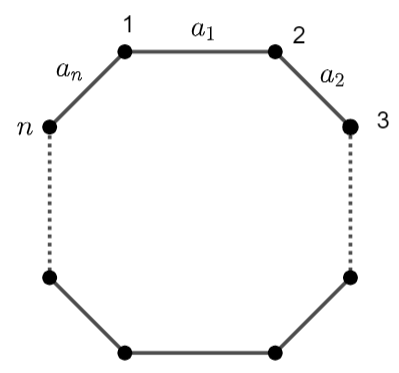
\includegraphics[width=0.35\linewidth]{pictures/Cn.png}
    \caption{${\bf C_n}$}
    \label{Cn:image}
\end{figure}
\textbf{Твердження 2.}\\
Для відновлення $C_n$, $n\geq 5$ достатньо таких трьох підспектрів: $\sigma({\bf C_n}-\{2\})$, $\sigma({\bf C_n}-\{2,3\})$,  $\sigma({\bf C_n}-\{5,...,n\})$.